\section{Iteration 2: Binary IR vs. Valued IR}
\sean{the term Binary IR and Valued IR can be refined.}
\subsection{Problem Statement and Goal}
With our first study, we learn that using IR to perform {\em coarse selection} can reduce the overall target selection time. A major reason for the improvement is because disambiguation is only needed 10\% of the time. 
%because in many cases there will be only one target in range and fine selection is not needed, and in cases where it’s needed, the list length has been effectively reduced. 
However, if the environment becomes denser, more disambiguation will be needed. And learning from Figure~\ref{fig:selection-time}B, we know the average results when disambiguation is involved is significantly increased. Hence our next research question becomes ``can we improve selection time in a dense environment?''

\subsection{Technique}
Previously we only used IR reception as a signal for identifying potential targets. It's a binary value indicating whether a target has received IR signal or not. To further capture the user's attention, we believe that IR intensity at the receiver side can provide more information. The IR intensity falls when the distance between IR emitter and receiver increases as well as when the receiving angle increases. We have empirically measured the intensity distribution at the receiver side, and it's shown in Figure~\ref{fig:measurement}. \ben{still working on it, not sure how much value we will get out of it. Seems useful to support the argument of the benefit though.}

\begin{figure}[t]
\centering
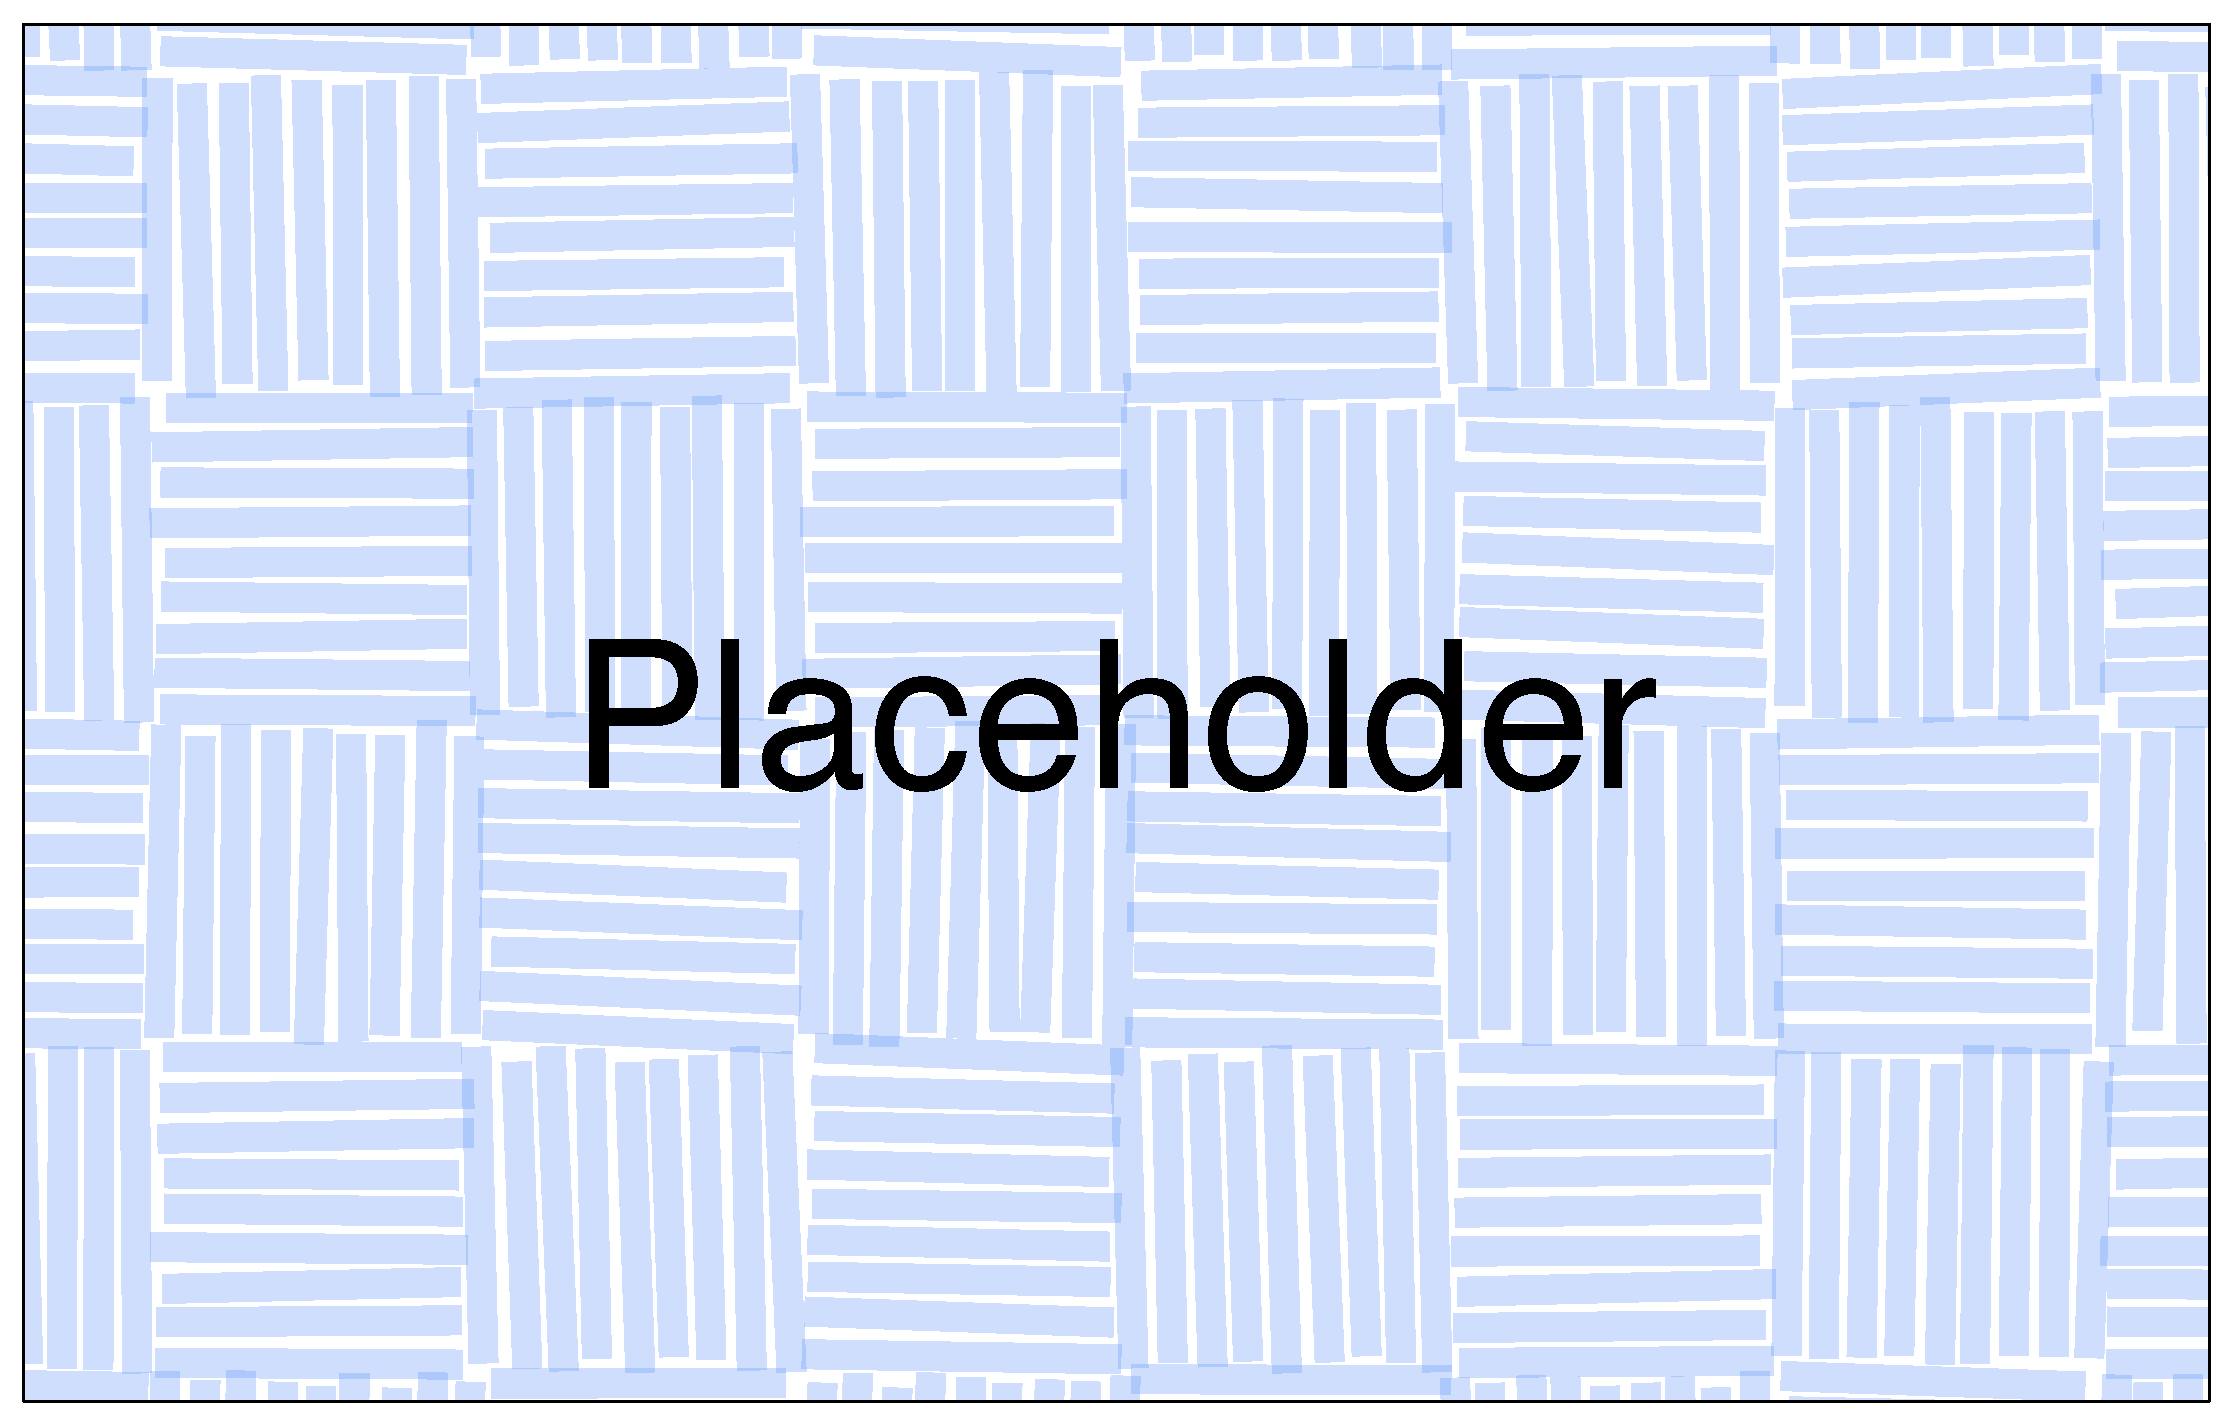
\includegraphics[width=0.9\columnwidth]{figures/placeholder.pdf}
\caption{placeholder for emperical measurement.}
\label{fig:measurement}
\end{figure}

From the measurement above we learned that the angular difference has a large effect on the intensity readings. In order to utilize the intensity, we have designed and 3D printed a repositional IR holder that can be clipped onto Glass. Thus, different users can adjust the emitter to align with their line of sight. \ben{need to mention in iteration 1 about the crappy tape}. 

\begin{figure}[t]
\centering
\includegraphics[width=0.9\columnwidth]{figures/tube_from_top.jpg}
\caption{The repositional IR holder.}
\label{fig:measurement}
\end{figure}



The intensity information is used in two ways:
\begin{enumerate}
\item When multiple targets have received IR signal and reported the intensity readings, we discard those whose intensities are significantly lower than the largest reading\footnote{In our current implementation, we empirically set it to be half, which is frequently used because it indicates a 3dB loss in the signal strength.}. Therefore, when there is only one target within line of sight, the IR intensity approach has the same behavior as the previous iteration - no disambiguation is needed. When the environment turns denser, the new design can filter some peripheral targets out, making the chances of entering disambiguation lower.
\item When disambiguation is still needed, meaning that multiple targets have relatively close intensity values, the system sorts the disambiguation list according to the IR intensity, from strongest to weakest. This will help us reduce the $t_{disambiguation}$ significantly if the first one appears matches the actual target.
\end{enumerate}

We seek to quantify the improvement of such design and performed another user study to compare the {\em Binary IR} and {\em Valued IR} approaches. For this study, we aim to discover the performances at a denser environment. Thus, we take the 10 nodes and set it up in a smaller area (see Figure~\ref{fig:study-layout2}). In total, we have 10 users for this study, and each user performs 30 target acquisition tasks for each approach. Similarly to our first within-subject study, half of them perform {\em Binary IR} first and the other half {\em Valued IR} first.

\begin{figure}[t]
\centering
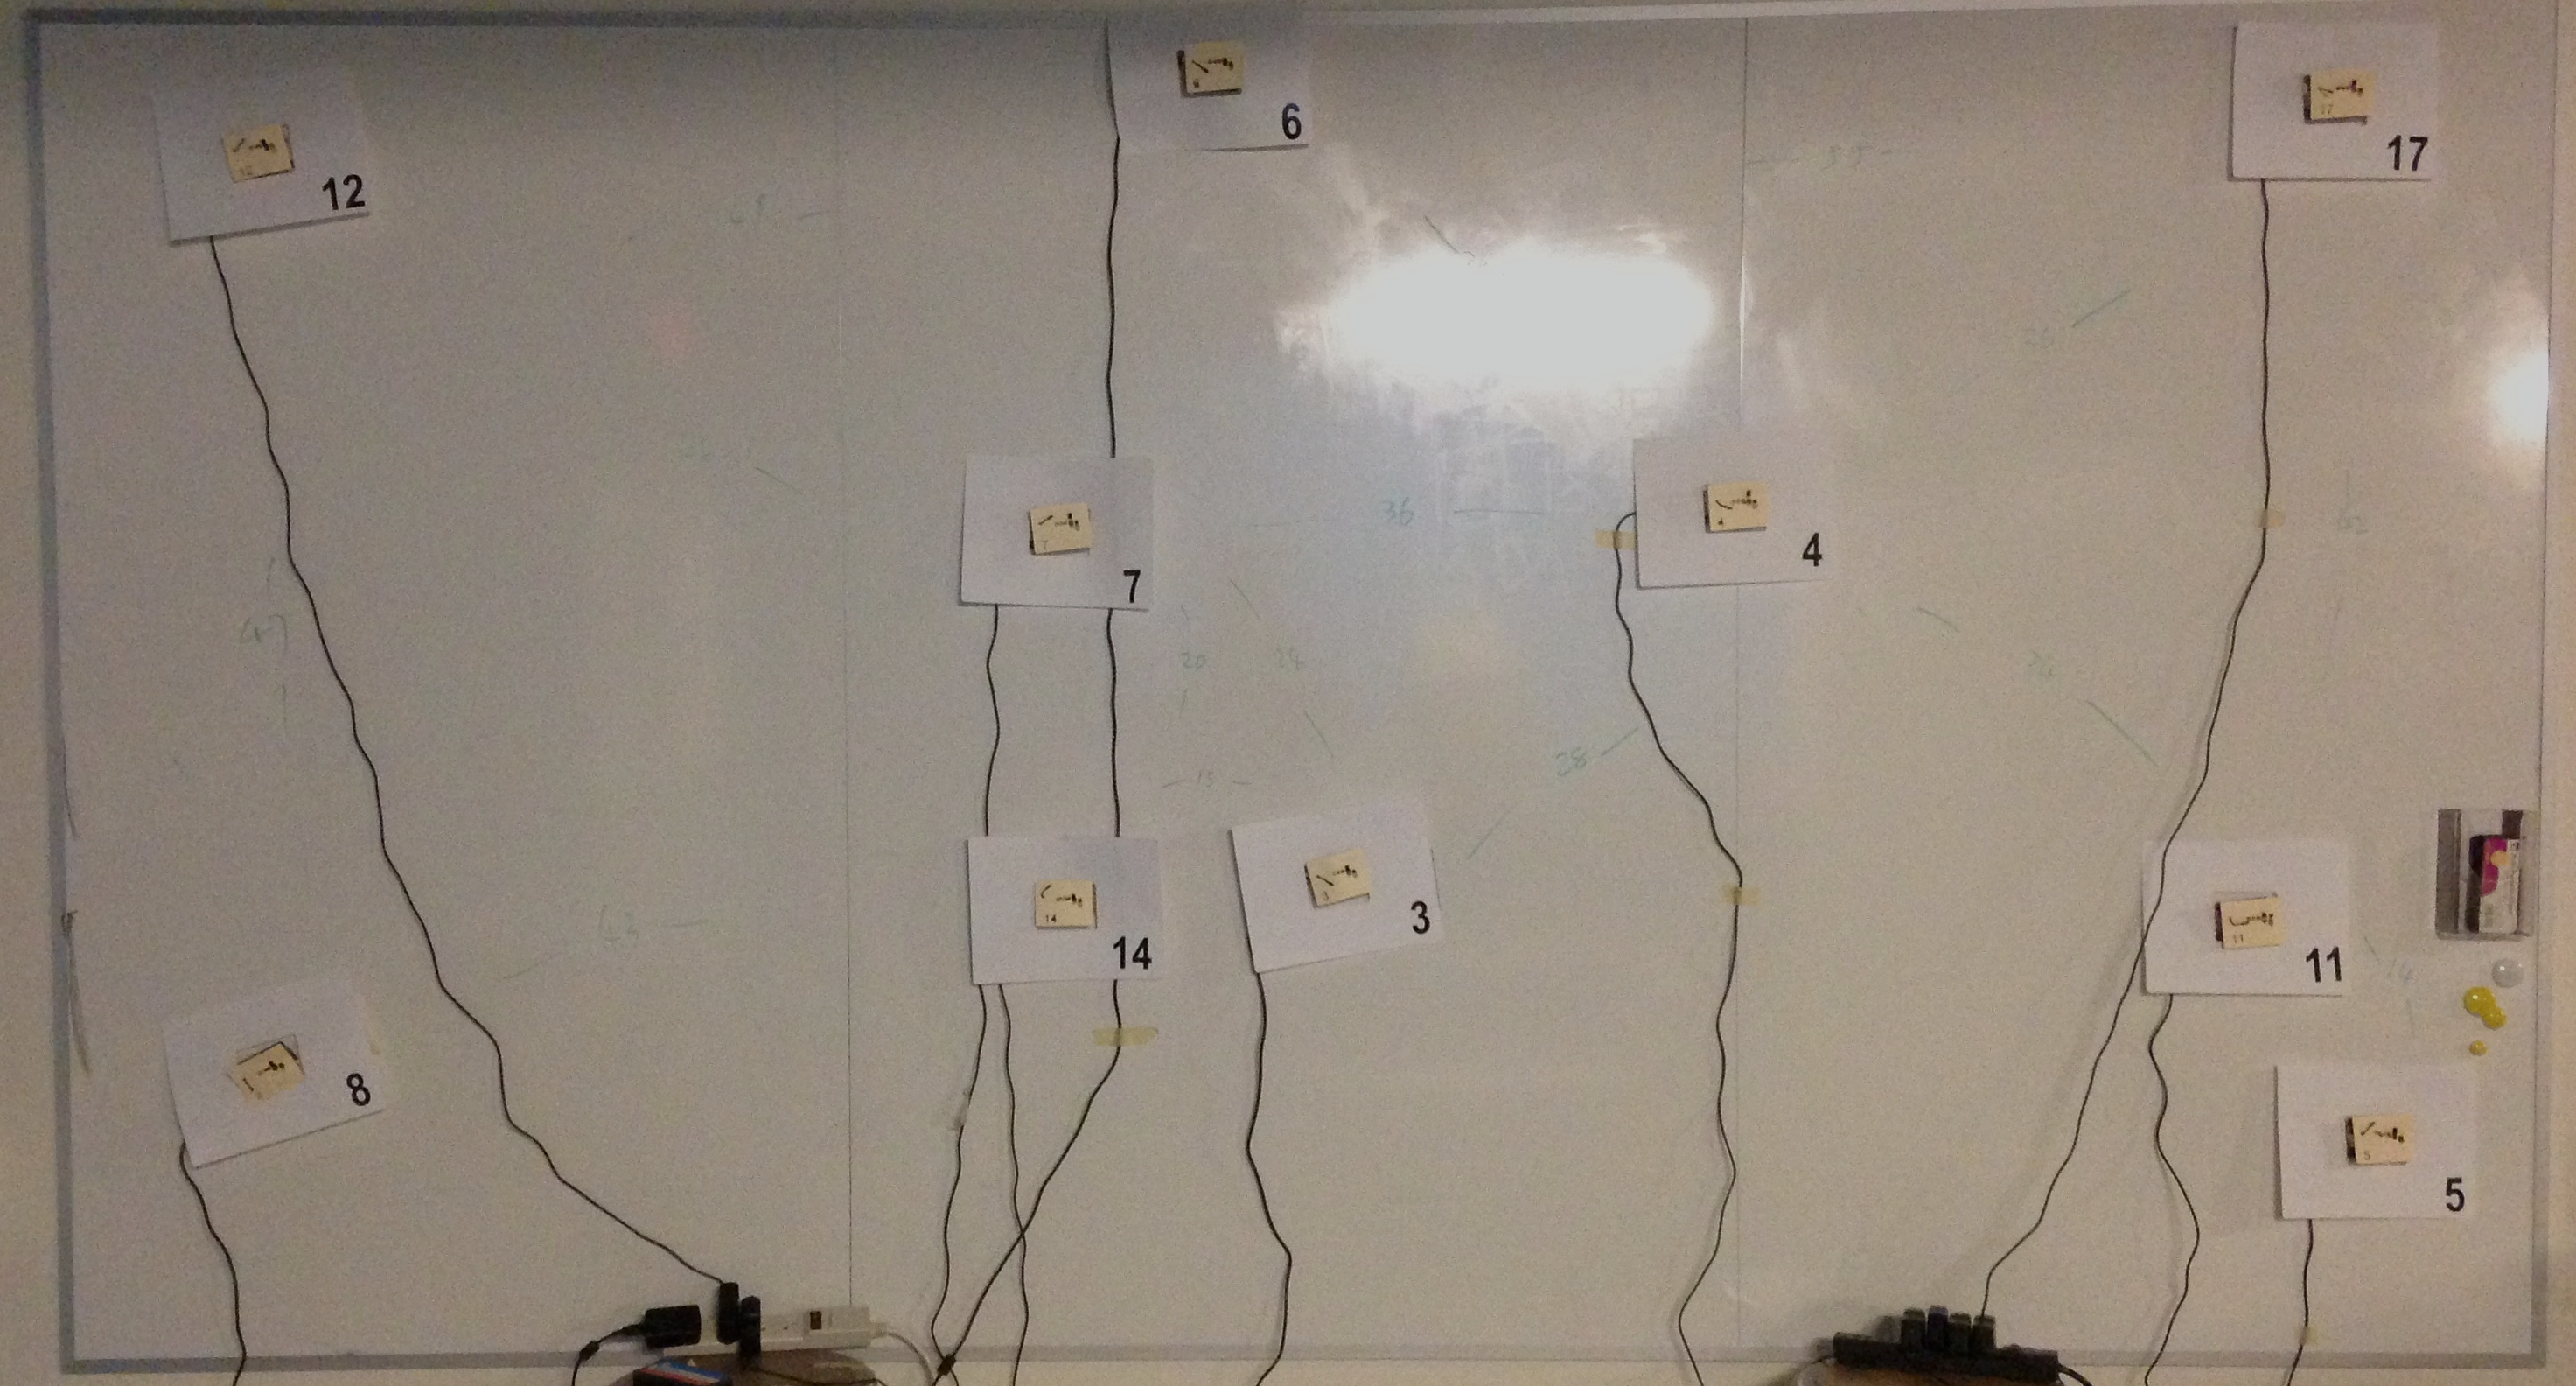
\includegraphics[width=0.9\columnwidth]{figures/study-layout2.jpg}
\caption{The current environment setup \ben{needs annotation and a better photo.}.}
\label{fig:study-layout2}
\end{figure}

% new study results
% ceiling(c(nrow(name), nrow(name_multiple), wrong_guess, wrong_percentage * 100))
% intensity
%  300 167  74  45
% name
%  300 225 145  65

%% first one
%% 
%             Outcome 1	Outcome 2	     Total
% Group 1 	167	133	300
% Group 2	225	75	300
% Total	        392	208	600
%% Chi squared equals 24.755 with 1 degrees of freedom. 
%%  The two-tailed P value is less than 0.0001


% 	    Outcome 1	Outcome 2	     Total
% Group 1	74	93	167
% Group 2	145	80	225
% Total	        219	173	392
% Chi squared equals 15.758 with 1 degrees of freedom. 
%   The two-tailed P value is less than 0.0001




\subsection{Evaluation}
Below is a summary of the study result.
\begin{enumerate}
\item Among the 300 trials in {\em Binary IR} condition, there are 225 times when disambiguation is needed. In {\em Valued IR} condition, only 167 out of 300 trials need disambiguation. We perform a Chi-square test on this result and the result is $\chi^2(1) = 24.755$, $p < 0.0001$. This demonstrates that the new approach successfully reduces the chances where disambiguation is needed.
\item In the cases when disambiguation is inevitable, the {\em Valued IR} will sort the list based on the intensity reading. As a result, out of the 167 times when disambiguation is involved, {\em Valued IR} sorts the desired target as the first one in the list 93 times (roughly 55\%). In comparison, for {\em Binary IR}, only 80 out of 219 (35\%) times can the user find the desired target first in the list. Again a Chi-square test demonstrates the statistical difference (with $\chi^2(1) = 15.758$, $p < 0.0001$. 
\end{enumerate}

Such gain can be seen from Figure~\ref{fig:study2} where the overall target acquisition time is obtained. The average time is 4.31 seconds and 3.64 second for {\em Binary IR} and {\em Valued IR}, respectively; and a t-test shows that they are also significantly different $t(555)=3.2945$, $p=0.001$.

%  t.test(name$complete, intensity$complete)

% 	Welch Two Sample t-test

% data:  name$complete and intensity$complete
% t = 3.2945, df = 555.272, p-value = 0.001049
% alternative hypothesis: true difference in means is not equal to 0
% 95 percent confidence interval:
%  0.2707875 1.0704747
% sample estimates:
% mean of x mean of y 
%  4.311340  3.640709 

\begin{figure}[t]
\centering
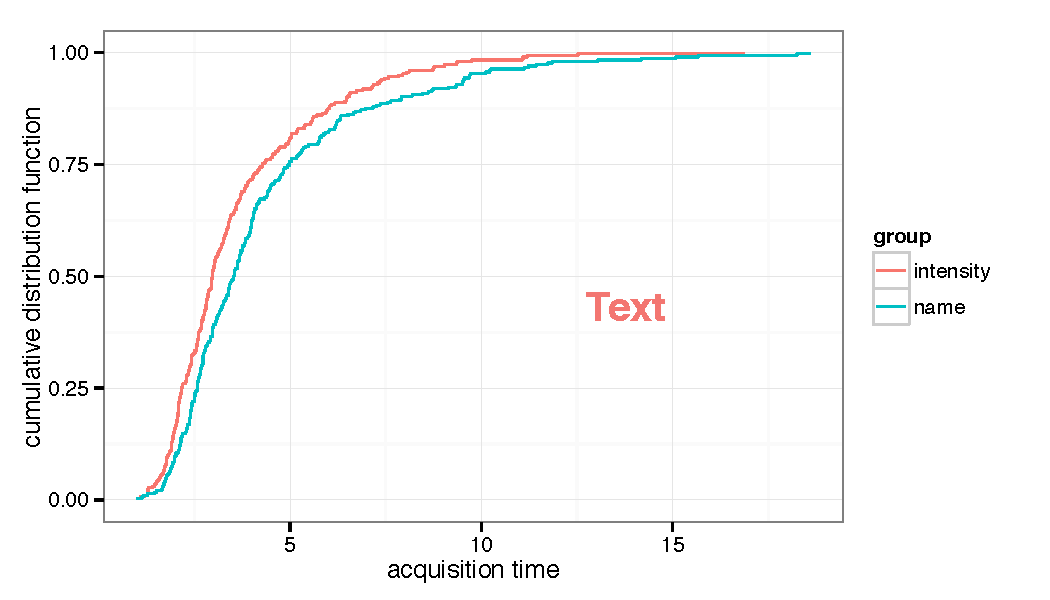
\includegraphics[width=0.9\columnwidth]{figures/study2_time.pdf}
\caption{The target acquisition of in {\em Valued IR} and {\em Binary IR} condition.}
\label{fig:study2}
\end{figure}

However, one side effect that we have observed in this approach is that the {\em Valued IR} sometimes eliminates the desired target during the {\em coarse selection} stage. The rate is not high (13 out of 300 cases, 4.3\%), but this is the trade-off for the overall faster acquisition time.

%%% Local Variables: 
%%% mode: latex
%%% TeX-master: "uist14"
%%% End: 
